%% ------------------------------------------------------------------------- %%
\chapter{Introdução}
\label{cap:introducao}

Princípios que ganharam destaque com os métodos ágeis de desenvolvimento
de software vêm expandindo suas fronteiras e se aderindo a outros aspectos
do desenvolvimento de um produto. A importância da \emph{iteratividade}
é um desses princípios que se tornam evidentes em abordagens modernas de
desenvolvimento de produtos, como o \emph{design thinking}~\cite{Brown2009DesignThinking},
ou em abordagens de modelos de negócios, como o \emph{lean startup}~\cite{Ries2011Lean}.
Um dos benefícios em se acelerar o ciclo de iterações é o aumento
de \emph{feedback} recebido, o que pode ser usado
para se redirecionar e refinar tanto o \emph{o que fazer}, 
quanto o \emph{como fazer}.

A implantação de um software é o
processo que vai da aquisição à
execução desse software~\cite{DEPL2006},
sendo que a \emph{aquisição} pode corresponder 
a um desenvolvimento interno na organização que irá implantar o software.
Na implantação de sistemas, 
o princípio de iteratividade
ganhou força com as ideias de entrega contínua de software~\cite{Humble2011Continuous},
o que é uma evolução da prática de integração contínua~\cite{Duvall2007Integration}, 
já incorporada à métodos ágeis como o XP~\cite{Beck1999XP}.
Entregar software continuamente significa que normalmente cada \emph{commit}
no código-fonte, que seja aprovado por uma bateria de testes,
corresponde a uma versão potencialmente implantável.
E a capacidade de se implantar software continuamente é passo fundamental
para o lançamento constante de novas versões de um sistema.

Serviços web possibilitam a comunicação interoperável entre máquinas pela rede~\cite{W3C2004WS}
e podem ser compostos para implementar sofisticados processos de negócios~\cite{Papazoglou2007State}.
Especialistas do setor aéreo, por exemplo, propõem o uso de composições de serviços
para automatizar os processos de negócios entre diferentes organizações
que coabitam um aeroporto~\cite{Choreos2012D6.2}.
Considerando os atuais números relativos a grandes
aeroportos\footnote{Heathrow [\url{http://www.heathrowairport.com}] em Londres, por exemplo, 
possui mais de 80 compahias aéreas, 190.000 passageiros por dia (picos de 230.000),
6.000 empregados, 1.000 pousos e decolagens por dia, e 40 serviços de refeição.}
e o crescimento futuro desses números, espera-se que
composições de serviços envolvam um grande número de participantes,
conforme já sugerido por 
pesquisadores~\cite{Valerie2011FutureInternet,Papadimitriou2009FutureInternet}.

No entanto, o desenvolvimento de colaborações entre serviços 
trazem desafios para a formulação de mecanismos que funcionem, 
escalem e que sejam eficientemente implementados 
em um ambiente distribuído de \emph{grande escala}~\cite{Steen2011VeryLarge}.
Nesse cenário de grande escala,
o processo de implantação enfrenta diversas dificuldades, 
tais como falhas corriqueiras na infraestrutura, 
heterogeneidade tecnológica, 
distribuição do sistema por diferentes organizações
e atualização frequente dos serviços em operação.
Com essas dificuldades, torna-se muito difícil manter a escalabilidade do processo de implantação
sem a utilização de um processo de implantação totalmente automatizado,
uma vez que processos de implantação manuais tendem a ser
morosos, propensos a erros e não reprodutíveis, principalmente
na implantação de sistemas distribuídos~\cite{Dolstra2005Configuration}.

Esses desafios podem ser tratados por soluções \emph{ad-hoc},
nas quais um processo de implantação é automatizado tendo em vista
uma composição de serviço específica.
Contudo, esse caminho leva ao baixo reúso de soluções
dentro de uma organização e entre as organizações participantes.
Outro caminho é a utilização de soluções baseadas em um \emph{middleware},
que resolvem os problemas comuns de implantação,
fornecendo soluções potencialmente mais sofisticadas e mais bem testadas.
Isso ocorre pois contribuidores interessados no problema de implantação
trabalham juntos para fornecer uma infraestrutura mais robusta,
enquanto usuários do middleware escrevem código menor e mais simples
para automatizar o processo de implantação de composições específicas.
Embora apresentem vantagens, sistemas apoiados por middleware
também apresentam desvantagens, principalmente no que diz respeito
às restrições impostas ao desenvolvimento da aplicação.

Nesta dissertação, estudamos o processo de implantação automatizada baseado em um middleware. 
Investigamos o quanto e como essa opção
contribui à implantação de composições de serviço de grande escala
quando confrontada com soluções \emph{ad-hoc}.
Para responder à questão colocada, nosso objetivo nesta dissertação é 
projetar, implementar e avaliar
um middleware que forneça suporte à implantação automatizada de composições de serviços web
de grande escala.
Esse middleware, quando comparado a soluções \emph{ad-hoc},
deve \emph{facilitar} a automação da implantação de composições diversas.
Nesse caso, \emph{facilitar} significa reduzir o tempo e/ou quantidade de trabalho
para a codificação e/ou aplicação da solução de implantação.
Avaliamos o tempo em homens-horas e a quantidade de trabalho
em linhas de código.
Também espera-se que a automação do processo fornecida por esse middleware
contribua para a escalabilidade do processo de implantação.
Nesse caso, ser escalável significa ser capaz de implantar uma maior quantidade
de serviços sem aumentar o tempo de implantação, dado que se aumente também,
proporcionalmente, a quantidade de servidores disponíveis para hospedar esses serviços.

A computação em nuvem possibilita o acesso a um conjunto compartilhado de recursos computacionais que podem ser providos rapidamente \cite{Nist2011Cloud}.
A gerência programática de recursos virtualizados, fornecidos pela nuvem, favorece a criação de processos totalmente automatizados para a implantação de sistemas \cite{Humble2011Continuous}.   
Além disso, sistemas distribuídos já estão migrando para ambientes de nuvem, onde são compostos e mantidos de modo descentralizado por várias organizações \cite{Steen2011VeryLarge}.
Baseando-se nessas considerações, nosso middleware foi projetado em função dos modelos de computação em nuvem.

O middleware desenvolvido no contexto deste trabalho é o CHOReOS \ee 
\footnote{\url{http://ccsl.ime.usp.br/EnactmentEngine}} (EE),
que funciona no modelo de Plataforma como um Serviço (PaaS), 
um dos modelos de funcionamento da computação em nuvem.
O EE fornece uma API remota para disparar o processo de implantação.
Essa API recebe uma especificação declarativa da composição a ser implantada.
O EE interpreta a especificação recebida e realiza as tarefas de implantação
em um conjunto de máquinas virtuais.
Essas máquinas virtuais são criadas por provedores de infraestrutura que funcionam
de acordo com o modelo de computação em nuvem denominado Infraestrutura como um Serviço (IaaS).
Ao fim da implantação, as composições de serviços estão disponíveis para serem consumidas
por usuários, operando no modelo de Software como um Serviço (SaaS).
A relação entre os modelos de computação em nuvem e nossa solução
pode ser observada na Figura~\ref{fig:modelos_nuvem}. 

\begin{figure}[!h]
  \centering
  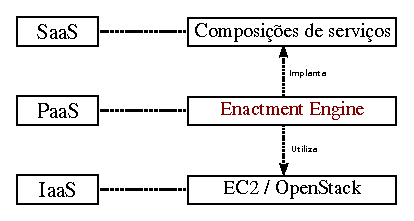
\includegraphics[width=.80\textwidth]{nuvem_modelos.pdf} 
  \caption{Modelos da computação em nuvem associadas ao CHOReOS \ee.}
  \label{fig:modelos_nuvem} 
\end{figure}

Esta pesquisa foi feita no contexto e com financiamento dos projetos CHOReOS\footnote{\url{http://www.choreos.eu}} e Baile\footnote{\url{http://ccsl.ime.usp.br/baile}}, que estudaram a aplicação de composições de serviços distribuídas, chamadas \emph{coreografias}, em ambientes de grande escala. O projeto CHOReOS, financiado pela Comissão Europeia e composto por diversas instituições acadêmicas e industriais da Europa conjuntamente com o IME-USP, objetivou desenvolver um processo dinâmico e centrado no usuário para o desenvolvimento de coreografias em um ambiente de escala ultra grande, no qual milhares de serviços são compostos e coordenados por um middleware distribuído. O projeto Baile, uma parceria entre IME-USP e HP Brasil, estudou a solução de problemas para o desenvolvimento de coreografias, como a adoção de Desenvolvimento Guiado por Testes (TDD) no contexto de coreografias e o suporte da Computação em Nuvem à implantação de coreografias. 

As contribuições deste trabalho são: 

\begin{itemize}
\item A implementação de um middleware que possibilita a implantação automatizada de composições de serviços. Além de possuir aplicabilidade direta para profissionais da indústria, nosso middleware facilita a condução de avaliações empíricas ligadas à implantação de composições de serviço, tendo assim potencial para alavancar diversas outras pesquisas sobre composições de serviços. 
\item Uma comparação, baseada na literatura e em evidências empíricas, entre soluções de implantação automatizada implementadas de forma \emph{ad-hoc} e implementadas com suporte por middleware.
\end{itemize}

Os esforços iniciais desta pesquisa, focando na implantação de composições de serviços em um ambiente de computação em nuvem, ainda sem considerar os desafios de grande escala, resultaram na seguinte publicação: \\

\begin{shadowblock}{15cm}
Leonardo Leite, Nelson Lago, Marco Aurélio Gerosa e Fabio Kon. Um Middleware para Encenação Automatizada de Coreografias de Serviços Web em Ambientes de Computação em Nuvem. Em \emph{31º Simpósio Brasileiro de Redes de Computadores e Sistemas Distribuídos (SBRC)}, 2013.
\end{shadowblock}

Durante o desenvolvimento do software Enactment Engine, o autor desta dissertação utilizou nos testes de unidade um padrão de software que foi documentado em um artigo de sua autoria: \\

\begin{shadowblock}{15cm}
Leonardo Leite. Fábrica dinâmica de dublês: testando classes que possuem dependências não injetáveis. Em \emph{Miniconferência Latino-Americana de Linguagens de Padrões para Programação (MiniPlop Brasil)}, 2013.
\end{shadowblock}

Ainda no contexto deste mestrado, foi realizado um estudo sobre adaptação dinâmica de coreografias, o que resultou na publicação do seguinte artigo: \\ 

\begin{shadowblock}{15cm}
Leonardo Leite, Gustavo Oliva, Guilherme Nogueira, Marco Aurélio Gerosa, Fabio Kon e Dejan Milojicic. A systematic literature review of service choreography adaptation. \emph{Service Oriented Computing and Applications}, 3(7):201--218, 2013.
\end{shadowblock}


Esta dissertação foi organizada da seguinte forma: as fundamentações teóricas sobre composição de serviços, o processo de implantação e a computação em nuvem são apresentadas no Capítulo~\ref{cap:conceitos}. No Capítulo~\ref{cap:relacionados}, apresentamos os trabalhos relacionados. No Capítulo~\ref{cap:solucao}, apresentamos o CHOReOS \ee, discutindo como suas características arquiteturais e de implementação auxiliam na implantação de composições de grande escala. A comparação do EE com soluções \emph{ad-hoc}, bem como sua avaliação de desempenho e escalabilidade, são apresentadas no Capítulo~\ref{cap:avaliacao}. Por fim, no Capítulo~\ref{cap:conclusoes}, apresentamos nossas conclusões.

%% ------------------------------------------------------------------------- %%
% Intro deve ter:
% background
% problema de pesquisa
% questão de pesquisa
% hipótese (?)
% objetivo de pesquisa
% contribuições



